%!TEX root = ../template.tex
%%%%%%%%%%%%%%%%%%%%%%%%%%%%%%%%%%%%%%%%%%%%%%%%%%%%%%%%%%%%%%%%%%%%
%% chapter2.tex
%% NOVA thesis document file
%%
%% Chapter with the template manual
%%%%%%%%%%%%%%%%%%%%%%%%%%%%%%%%%%%%%%%%%%%%%%%%%%%%%%%%%%%%%%%%%%%%

\typeout{NT FILE chapter2.tex}

\chapter{Theoretical and Technical Concepts}
\label{cha:technical_concepts}

\begin{figure}[htbp]
	\centering
	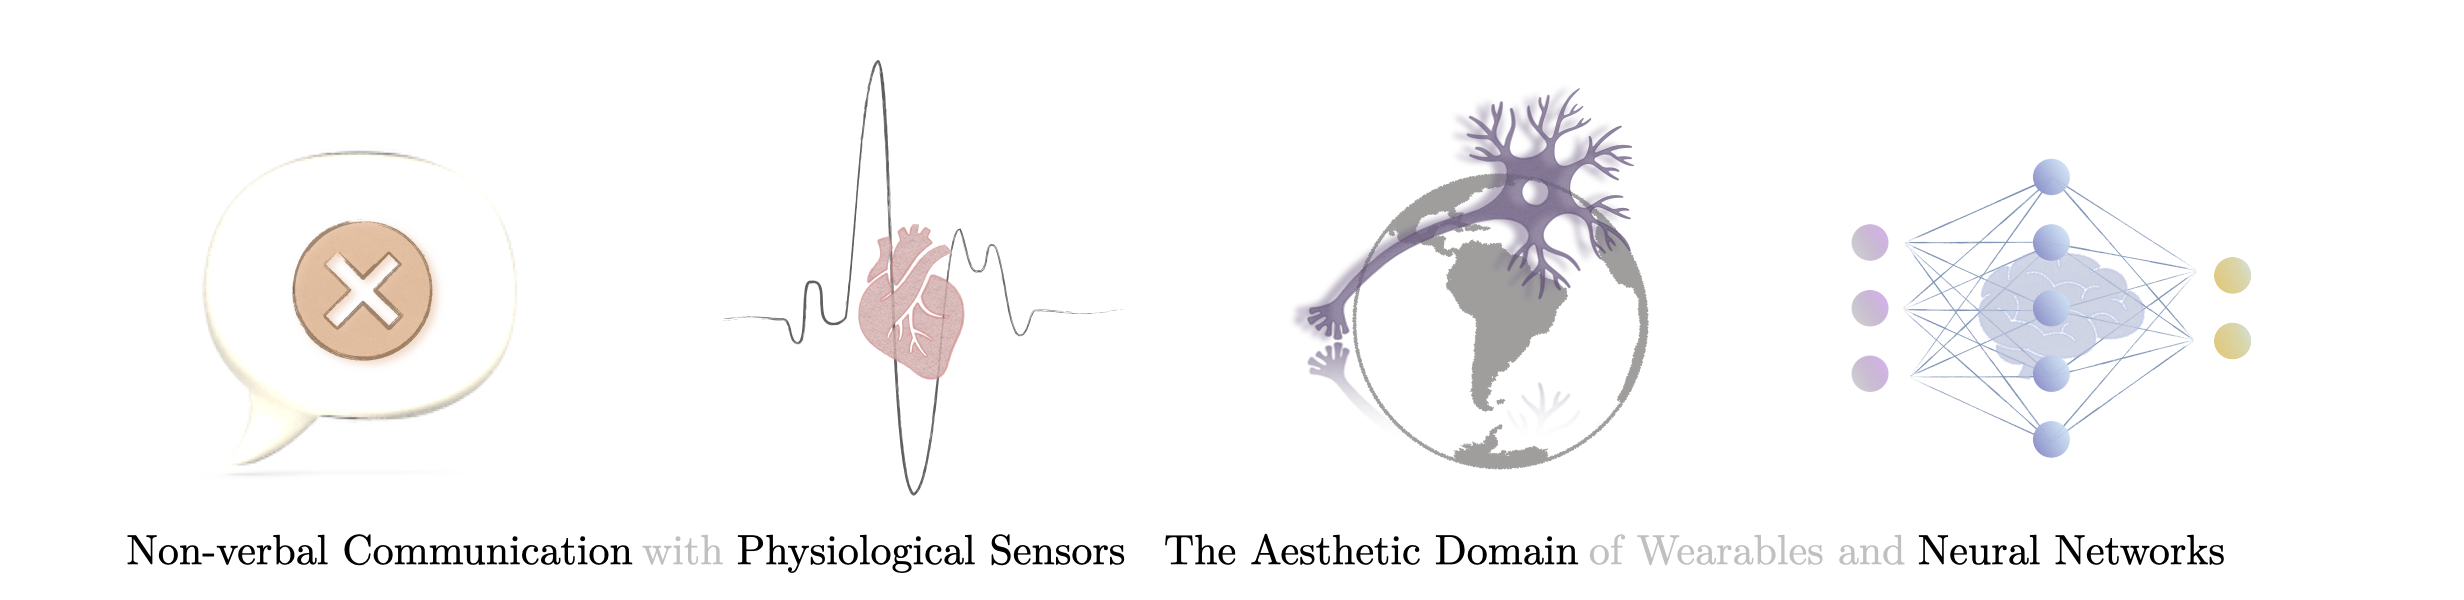
\includegraphics[width=\textwidth]{Chapters/Figures/background/sec2_title_constructs_alpha_2.png}
	\caption{Title constructs illustrated}
	\label{fig:title_constructs}
\end{figure}

In the following section, we initiate the theoretical framing directed towards the thesis research goals. We begin by breaking down the thesis title into four constructs that are used to establish the major themes of the research (shown in Figure \ref{fig:title_constructs}, each accompanied by preliminary definitions as well as key references present in the literature. We aim to address some of the commonalities between these that help to unify these concepts into a common research goal. This framework is further supplemented with an overview of key principles taken from other complementary fields, concluding with a proposed criteria for aesthetic evaluation.

\section{Non-verbal Communication with Physiological Sensors: The Aesthetic Domain of Biosignals and Neural Networks}
\label{sec:title_constructs}


\subsection{Non-Verbal Communication}

Non-verbal communication is an umbrella term used to distinguish modalities of interpersonal exchange that are independent of speech, many of which are unconsciously transmitted during social relations, this encompasses a variety of modalities that convey emotions, feelings, and messages. Behavioural analysis grounded in psychology research calls attention to the emotional information disclosed by non-verbal social cues, in particular, actions that are involuntary. Computing and Physiology researcher Alex Petland frames these as \textit{Honest Signals} to articulate a level of emotional authenticity while complimentary studies note the permitted degree of ambiguity.

\textit{“The unconscious quality of particular informative non-verbal behavioural cues grants a level of authenticity”} \citeauthor{pentland_honest_2010} \cite{pentland_honest_2010}
% Pentland et al. 2010. Honest Signals: How They Shape Our World

\subsection{Physiological Sensors}

Physiological signals provide a measurement of biophysical, biomechanical and bioelectrical changes that occur from within the body. These data streams can be used to validate semantic emotional descriptors based on valence and arousal measurements, linked to the user’s involuntary reactions transmitted by the Autonomic Nervous System (ANS) \cite{levenson_autonomic_2014,shu_review_2018}. These are widely used to monitor a plethora of non-verbal social cues, measuring the ‘invisible’ internal signals that are otherwise not explicitly perceived.

Non-verbal behaviour is commonly associated with “body language”, aspects such as posture, gaze and other observable traits. But how about bodily signals that are invisible from a third-person perspective? Signals acquired using physiological sensors (or biosignals) are capable of monitoring these internal changes, that can be associated with an emotional response, typically in accordance with a measure of arousal, that operates on a linear scale.

\textit{“In other words, nonverbal behavioural cues are the physical, machine detectable evidence of affective phenomena not otherwise accessible to experience, an ideal point for technology and human sciences to meet.”} \citeauthor{vinciarelli_towards_2011} \cite{vinciarelli_towards_2011}
% Vinciarelli et al. ’Towards a Technology of Nonverbal Communication: Vocal Behavior in Social and Affective Phenomena’

% These signals are traditionally represented as a low-dimensional format. For example, one ECG sensor will pick up a uniform series of amplitudes over time, isolating the electrical response from the heart, separated from the surroundings

\subsection{The Aesthetic Domain}

To put forward such a heavily loaded concept, we can reduce aesthetics down to its literal derivative of \textit{aístesis}, which describes the process of perceiving through sensory engagement. Whilst this phenomenon is continually re-evaluated, it can be assumed to operate on a scale of order and complexity. This is essentially how we as humans are able to perceive new kinds of information contained in our surroundings, reducing to a meaningful inference, through a process of learning as a result of personal experiences. From this, we consider ambiguity as an affordance for expressive exchange. In \textit{Two Modernist Approaches to Linking Art and Science}, Eric R. Kandel ties relevance to the art history concept of the beholder's share to the biological understanding of the human mind \cite{kandel_two_2013}.

\textit{"Human emotional life is rich; we can experience a huge number of emotions, possibly a continuum, not just a few for which we have words, like fear, sadness, joy, etc."} \citeauthor{perlovsky_aesthetic_2014} \cite{perlovsky_aesthetic_2014}

% Kris & Kaplan. 1952. Aesthetic Ambiguity

\subsection{Neural Networks}

An artificial neural network aims to simulate the core functions of the human brain, used to define complex input-output patterns, using previously learned information to comprehend sensory inputs. Combined with the other constructs, we consider the human-like qualities of Artificial Neural Networks (ANNs) as the technical foundation for emotional engagement with physiological data. As modern data science practices have already validated neural networks as an effective method for associating human-understandable contexts to otherwise ambiguous sensor data \cite{bota_review_2019}, we reflect upon human-centred augmentations by which the user is immersed in the learning process.

\textit{"Treating embodied knowledge as something that cannot be accessed directly and only through examples of action (treating the learning algorithm as a “black box”) is therefore missing a lot.” }

\citeauthor{gillies_understanding_2019} \cite{gillies_understanding_2019}
% M. Gillies, ‘Understanding the Role of Interactive Machine Learning in Movement Interaction Design’


\section{Physiological Signals}

\subsection{Physiological Signal Categories}
\label{subsec:catagories}

In this document, we will cover a range of physiological signals in the context of potential interaction modalities. Physiological signals can be categorised according to the origin of the activity that is being recorded from the body \cite{enderle_introduction_2012}. The signals we will be assessing and comparing in this work are defined as bioelectrical and biomechanical. Bioelectrical signals provide a measurement of the electric and electromagnetic fields produced by living cells. Examples include Electromyography (EMG), Electrocardiogram (ECG), and Electrodermal activity (EDA) \cite{malmivuo_bioelectromagnetismprinciples_1995}. Biomechanical signals on the other hand measure the physical forces produced by or applied to the cells, tissues and organs. These include respiratory cycles and acceleration of the limbs \cite{guerreiro_bitalino_2013, pacelli_sensing_2006}. The complete list of categories based on anatomical origin is comprised of biomagnetic, biochemical, bioacoustic and biooptical signals. For more detailed information on physiological signals, we may refer the reader to \cite{webb_principles_2018}

\subsection{Controllability of Signals}

We take into account the controllability a subject has on a given physiological response, depending on the source, which can be classified as Voluntary, Indirect or Involuntary. Through Voluntary sources, the user can intentionally manipulate the signal with a high degree of freedom. These include, for example, muscle contractions or displacement of joints, activities that are associated with the somatic nervous system. Indirect (or Mixed) sources grant the user partial control whereas Involuntary sources indicate that there's almost no control over the outcome \cite{da_silva_biosignal_2017}. Involuntary sources are generally assumed to be transmitted from the autonomic nervous system as they occur without conscious control \cite{lenman_human_1975}.

Movement is normally categorised as a visible and voluntary action in the scope of physiological signals, and understandably so when compared to internal functions receptive to the ANS, such as cardiovascular activity. We aim to support the persuasion that many non-verbal behaviours do in fact materialise as involuntary motor actions \cite{haueisen_involuntary_2001} or even spontaneous micro-gestures \cite{chen_analyze_2019}, those so subtle that they can be difficult to perceive without any technological intervention, such as body-worn sensors \cite{jensenius_exploring_2017}.

% \subsection{Electromyography}

% \subsection{Electrocardiography}

% \subsection{Electrodermal activity}

% \subsection{Transdisciplinary Research Culture}
\subsection{Applications and Research}

Physiological sensing is studied prominently under the interdisciplinary field of biomedical engineering. This prides itself on pulling new perspectives from research fields such as electronics, programming, humanities, culture and psychology, and as such, invites specialists from alternative disciplines to validate insights outside of traditional practices \cite{enderle_introduction_2012}. For example, in affective computing research, the study of human psychology is vital for understanding the detection and regulation of emotions using technology. The term lends itself towards a vast selection of applications and research topics, to an extent that is impressive without doubt, but at the expense of obscurity when trying to determine a meaning that is inclusive. For example, biomedical engineering may be rightfully allocated to the production of prosthetic devices intended for physical rehabilitation \cite{valentinuzzi_physical_2019}, while on the other hand, it serves as a relevant label for say, a biofeedback system design for guided meditation \cite{foo_soft_2020}. What binds these distinct functions can be owed to the appropriation of biomedical technology and data, which can be divided into two major essential categories: physiological sensors and actuators.

\textbf{Sensors}: These are the components that are responsible for acquiring physiological signals from the body, purposed to measure the specific bodily processes that occur. Section \ref{cha:Preliminary_Actions} provides a general overview of the common types of sensor modalities as well as their affordances.

\textbf{Actuators}: This describes some form of output mechanism that is being manipulated by the sensor data. The process in which we perceive this representation of physiological activity describes the foundation of biofeedback. In some design contexts, such actuation systems may be referred to as interactive artefacts.

As we begin to appreciate the value of such collaborations outside of the strictly medical domain, we will present our research efforts to continuously defend the inclusion of aesthetics, primarily in the scope of emotional modelling technology, but also in the broader scope of biomedical science. We foresee a co-benefit between the appropriation of physiologically-centred systems for artistic practices, and enhancing our sensory engagement with technology.
% And then, taking into consideration the novel aesthetic experiences to reconstruct our comprehension of live biodata as a resource for health and well-being,


\section{Non-verbal Cues and Social Signals}

A fundamental objective of this work is to explore methods of communicating emotional or affective states without a dependency on spoken language. Non-verbal communication is a term that encompasses a variety of modalities such as posture, physical gestures or facial expressions to convey emotions, feelings, and messages beyond the use of words \cite{knapp_nonverbal_2009, richmond_nonverbal_2011}. This can be interpreted to augment meaning alongside the verbal channel during an interaction, or by itself in circumstances where there are only non-verbal channels present.

Non-verbal signals can be described as communicative or informative. A signal is produced consciously in an effort to convey a specific meaning that is communicative. On the other hand, when the user emits signals unconsciously, without an intended meaning, it is informative \cite{vinciarelli_towards_2011}. The unconscious quality of particular informative non-verbal behavioural cues grants a level of authenticity, advocating the label of \textit{honest signals} by Alex Pentland \cite{pentland_honest_2010}.

The field of Social Signal Processing (SSP) can be tied to the increased importance of emotional sensibility covered in third-wave HCI research \cite{cristescu_emotions_2008}. Social Signal Processing revolves around the monitoring of non-verbal behaviour to analyse social interactions. The attention directed towards non-verbal communication can be justified as a method of extracting social signals that are hard-wired in the human brain \cite{vinciarelli_social_2009-1}.

\section{The Embodiment of Emotions, A Theoretical Primer}
\label{background:ebodiment_emotions}

The association between emotions and bodily expression in humans and animals was first described by Darwin \cite{darwin_expression_2013}, which has been followed by numerous studies in social psychology, human development, and more recently HCI \cite{alaoui_movement_2012, gillies_creating_2018, fdili_alaoui_strategies_2015} to address the communication of emotions from the human body \cite{gunes_lab_2008}. In this work, we will be working with the existing non-verbal modalities of gesture and posture, which are considered aspects of kinesics. They are both executed from the body and have the capacity to transmit social messages, but can be differentiated by their degree of intentionally and kinematic quality. Gestures are often (though not always) associated with movement and classed as communicative, as they are performed consciously \cite{vinciarelli_towards_2011}. A subcategory of gestures, known as \textit{adaptors} are performed unconsciously which may indicate changes in arousal or anxiety \cite{hans_kinesics_2015, neff_dont_2011}.

Social signals addressed from postures are commonly a result of unconscious behaviour making these amongst the most honest and reliable non-verbal cues according to Richmond and McCroskey \cite{richmond_nonverbal_2011}. In a seminal work on posture and communication, Scheflen proposes three main social messages to be extracted from an interaction \cite{scheflen_significance_1964}, to characterise the posture as inclusive or non-inclusive and to assess the level of engagement and rapport \cite{vinciarelli_social_2009}. Rapport can be associated with postural mimicry (or mirroring), which has been linked to smoother interactions and greater empathic understanding \cite{chartrand_chameleon_1999}.

This notion of the felt experience is compatible with various other philosophical theories proposed in the works of Merleau-Ponty \cite{merleau-ponty_phenomenology_2012}, James-Lang \cite{cannon_james-lange_1927}, Dewey's Aesthetics \cite{dewey_aesthetic_1950}, Lakoff \& Johnson \cite{lakoff_philosophy_1999} to name some, each serving deeply profound insights into perception and emotional life. We will refrain from describing individual details, but appreciate the cohering thread that runs among these is that emotions are not constrained to cognitive function alone, but rather taking resources from a corporeal body, responsive to enactive engagements.

\section{Somaesthetic Design}

If we concur with the baseline understanding of aesthetics that was defined in the title constructs (Section \ref{sec:title_constructs}), we can begin to formulate a concise understanding of this phenomenon when we recognise that aesthetic perception is not restricted to our 5 primary sense organs. Shusterman's philosophy expresses the importance of our entire body, and how this has been used not just to perceive, but how one interacts with their surroundings \cite{shusterman_body_2008}. Through Shusterman’s (Somaesthetic) theory, we can assure that aesthetic experiences are not strictly bound to a gallery setting or a formal artistic education, since the body is inherently capable of cultivating aesthetic value in everyday life. This ability is enhanced through performative practices, such as dance \cite{eric_c_mullis_performative_2006,shusterman_body_2012}.

Our approach is informed by the soma design process of Höök \cite{hook_designing_2018}, which “requires training your ability to aesthetically appreciate all your senses, but also to imagine through your senses, movements and material encounters” \cite{hook_soma_2019}. According to a soma design process, what takes form “is not only the digital and physical materials you use to build your interactive artifact with, but also the end-user's somas”. Somatic practitioners are known to intentionally disrupt habitual actions in order to decouple first and third-person perspectives, that is to comprehend their experiences from the outside-in. This was demonstrated in the "Collaborative Walking" exercise presented as part of the \textit{Move to Be Moved Workshop} \cite{hook_embracing_2018}, which was inspired by \citeauthor{loke_moving_2013}'s method \cite{loke_moving_2013}. This process leads us to understand the pinnacle function of technological intervention in contemporary Soma Design theory. Such methods have also been appropriated to support intercorporeal modes of being, \textit{"enhancing second-person perspectives, empathy, communication, and joint acts of perception and action"} \cite{turmo_vidal_designing_2021}.

% Other (more interesting) research communities share these ideas also
In the wider scope of body-centric HCI research, we include Somaesthetic design as an individual component amongst literature from other research communities, broadly speaking, studies of Moving Computing (MOCO) \cite{zhou_dance_2021} and Tanglable Embodied Interfaces (TEI) \cite{li_meta-analysis_2022}, to nominate some key examples. Soma and Somaesthetic design researchers have sustained a profound voice in pushing Affective Computing away from its traditional frameworks of emotion detection, but instead considering emotional experiences enriched by computer-mediated interaction, cultivating an alternative outlook that is now recognised as The Interactional Approach \citep{hook_affective_2009}. A plethora of articles and case studies can be found in the bibliography, with records dating back as far as the early 2000s that demonstrate and assert the relevance of this methodology (see Section \ref{affective_computng_lit_review} for more detail).

% \textit{Somatic connoisseurship} is granted to those that hold a comprehensive training and experience in one or more relevant body-centred practices, which certifies the appropriate facilitation of such activities to somatic laypersons.

% By navigating such theoretical progressions in alternative research fields, we can begin recognise patterns by which the adoption of aesthetics makes way for more emotionally relevant systems.

% \section{Interactional Design Perspective}

% - Traditional affective computing applications - informational View

% -An  interactional  perspective  on  design  will  not aim to detect a singular account of the “right” or “true” emotion  of  the  user  and  tell  them  about  it,  but  rather  make  emotional  experiences  available  for  reflection

% -When there is a continuous dialouge, we introduce affective loop experiences

% These concepts align with non-representational views of cognition, as it does not rely on a reductionist model of emotion.

\section {Parameters for Aesthetic Quality}

In the midst of cultural sensibility that's prevalent across HCI's third wave, we recognise that the Aesthetic Domain is truly a complex and multifaceted phenomenon that does not abide by traditional computational modelling, at least in an obvious way \cite{bardzell_interaction_2009, rentschler_innate_1999}. With aesthetics comes a permitted degree of ambiguity whereby the perceiver is responsible to construct their own emotional understanding of the artefact. This theory of meaning through engagement is discussed in further detail in Section \ref{lit_review:abstract}. We may clarify that ambiguity should not necessitate vagueness or obscurity, these being considered examples of poor communication. Rather, to understand the bridge between aesthetics and ambiguity as inherent components for individual expression by way of embodied metaphor \cite{dauden_roquet_body_2020,lakoff_metaphors_2003}. 

Complimentary to the core proposition for aesthetic representation as expressive mediation, the discussion of \textit{Aesthetic Emotions} sparks interest around the kinds of feelings that arise when engaging with artistic practices, opening up a rich space for emotional descriptors \cite{schindler_measuring_2017,fingerhut_aesthetic_2020}. A thorough enquiry into aesthetics and digital representation could rightfully be reserved for an entire thesis in itself, in which circumstance would there remain indeterminate concepts beyond its conclusion. To overcome an ever-expanding topic, we will begin by establishing a firm criteria based on two perceptual qualities:

\textbf{Spatial:} the distribution and organisation of distinct elements based on their relative position to one another and \textbf{Rhythmic:} the temporal presence for which something is produced and perceived, typically observed in regular intervals that are repeated.

\textbf{Spatial} representations may be identified in (a)symmetry, displacement and continuation in accordance with fundamental geometrical terminology \cite{mcmanus_symmetry_2005,boselie_general_1984}. Relating more closely to the anatomical frame, proprioception (or kinesthesia), refers to one's continual awareness to their individual body-parts according to sensory receptors that relay information about our body's spatial position \cite{lamkin-kennard_sensors_2019}. Taking this resource, the notion of orientational metaphor has been embedded into everyday communication, articulating the intersections that stand between embodied and emotional experiences \citep{gow_spatial_2001,zlatev_phenomenology_2010} (e.g. \textit{“My spirit rose”} and \textit{“I’m feeling down”})

\textbf{Rhythmic} qualities are determined by temporal patterns, examples of which are (a)synchrony, syncopation, entrainment and delay. We also point to the relevance of rhythm in the assessment of physiological regulation. Immediate examples of this are found in automatic functions such as respiratory and cardiac activity \cite{moser_phase_1995} which can even be seen working in tandem with one another \cite{scholkmann_pulse-respiration_2019}. Other processes occurring over longer time-frames, such as sleep cycles are also accountable to rhythmic patterns \cite{moser_why_2006}. The role of rhythmic motor activity has also been beneficial in the context of rehabilitation strategies \cite{fujii_role_2014}.

The spatial and rhythmic attributes described here stand as a very broad feature space, intended to remain generalisable across any kinds of mediums and modalities, as exemplified in the works documented in Chapters \ref{cha:Preliminary_Actions} and \ref{cha:case_studies}, demonstrating how rhythm and space are incorporated into sonic, visual and haptic forms of bodily representation. We appreciate in regardless that there persists an intuitive association that rhythmic qualities are commonly accepted as sonic representation whereas spatial distribution assumes to take on a visual geometric form. Nevertheless, we aim to balance these criteria throughout our investigation of different mediums. Additionally, features such as synchrony and entrainment can be used to characterise aspects of interpersonal behaviour that emerge during social interaction, as shown in previous studies focused on dyadic movement patterns being observed in a performance setting \cite{ward_sensing_2018} and those induced when listening to music \cite{scurto_entrain_2019,danielsen_moving_2015}.

To better clarify our understanding of the aesthetic domain, it’s important to depart from the contingency that aesthetic quality generally refers to something beautiful or pleasing to the senses, and therefore should not be biased toward positive emotion \cite{fingerhut_aesthetic_2020}. During the discussions that arise from the first case study, presented in Section \ref{case_studies:soma_chi}, we examine some of the prevalent themes associated with sensorial satisfaction, namely the convergences that lie between symmetry and asymmetry, as well as synchronous and asynchronous representation. The way in that we experience these sensorial stimuli can be characterised as spatial or temporal qualities respectively, which are given further attention in each of the latter two practical works presented in Sections \ref{case_studies:modi_dis} and \ref{case_studies:adse_ess}.
